\documentclass[tikz,border=2pt]{standalone}
\usepackage{amsmath}
\usepackage{pgfplots}
\pgfplotsset{compat=1.18}
\usetikzlibrary{arrows.meta}
\begin{document}
% Example 1: f(x)=x^2 on the compact [-1,2] attains min 0 at x=0 and max 4 at the end point x=2;
% on (0,2), which is not closed, f takes every value in (0,4) but neither 0 nor 4.
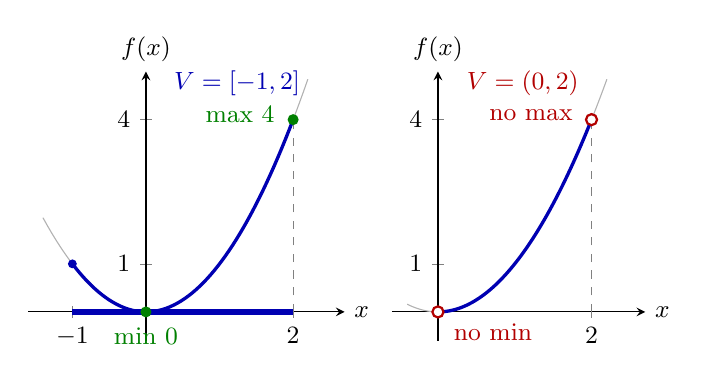
\begin{tikzpicture}[font=\small, >={Latex[length=2mm]}]
  \begin{axis}[
    name=left, axis lines=middle, xmin=-1.6, xmax=2.7, ymin=-0.6, ymax=5,
    xtick={-1,2}, ytick={1,4},
    xlabel={$x$}, ylabel={$f(x)$},
    xlabel style={anchor=west}, ylabel style={anchor=south},
    width=5.6cm, height=5cm, clip=false
    ]
    \addplot[gray!60, thin, domain=-1.4:2.2, samples=60] {x^2};
    \addplot[blue!70!black, very thick, domain=-1:2, samples=60] {x^2};
    \draw[blue!70!black, line width=2.2pt] (axis cs:-1,0) -- (axis cs:2,0);
    \draw[gray, thin, dashed] (axis cs:2,0) -- (axis cs:2,4);
    \fill[blue!70!black] (axis cs:-1,1) circle (1.6pt);
    \fill[green!50!black] (axis cs:0,0) circle (2pt) (axis cs:2,4) circle (2pt);
    \node[green!50!black, anchor=north] at (axis cs:0,-0.12) {min $0$};
    \node[blue!70!black, anchor=west] at (axis cs:0.25,4.75) {$V=[-1,2]$};
    \node[green!50!black, anchor=east] at (axis cs:1.88,4.1) {max $4$};
  \end{axis}
  \begin{axis}[
    at={(left.east)}, anchor=west, xshift=0.6cm,
    axis lines=middle, xmin=-0.6, xmax=2.7, ymin=-0.6, ymax=5,
    xtick={2}, ytick={1,4},
    xlabel={$x$}, ylabel={$f(x)$},
    xlabel style={anchor=west}, ylabel style={anchor=south},
    width=4.8cm, height=5cm, clip=false
    ]
    \addplot[gray!60, thin, domain=-0.4:2.2, samples=60] {x^2};
    \addplot[blue!70!black, very thick, domain=0:2, samples=60] {x^2};
    \draw[gray, thin, dashed] (axis cs:2,0) -- (axis cs:2,4);
    \draw[red!70!black, thick, fill=white] (axis cs:0,0) circle (2pt) (axis cs:2,4) circle (2pt);
    \node[red!70!black, anchor=north west] at (axis cs:0.08,-0.05) {no min};
    \node[red!70!black, anchor=east] at (axis cs:1.88,4.1) {no max};
    \node[red!70!black, anchor=west] at (axis cs:0.25,4.75) {$V=(0,2)$};
  \end{axis}
\end{tikzpicture}
\end{document}
